\begin{center}\scriptsize
    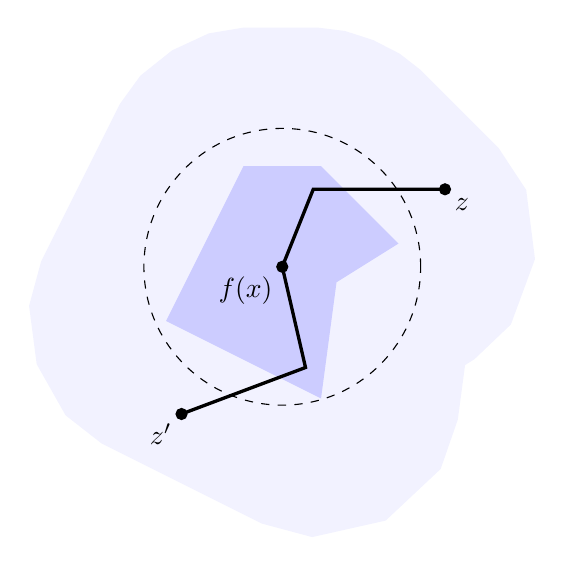
\begin{tikzpicture}[x=2.8em, y=2.8em]
    \draw[blue!05, line width = 10em, rounded corners] 
        (1,1) -- (3,0) -- (3.2,1.5) -- (4,2) -- (3,3) -- (2,3) -- (1,1) -- (3,0);
    \fill[fill=blue!20, very thick] 
        (1,1) -- (3,0) -- (3.2,1.5) -- (4,2) -- (3,3) -- (2,3) -- (1,1);
    \draw[very thick]
        (4.6,2.7) -- (2.9,2.7) -- (2.5,1.7) -- (2.8,0.4) -- (1.2,-0.2);
    \filldraw
        (2.5,1.7) circle(2pt) node[anchor=north east]{$f(x)$}
        (4.6,2.7) circle(2pt) node[anchor=north west]{$z$}
        (1.2,-.2) circle(2pt) node[anchor=north east]{$z'$};
    \draw[dashed]
        (2.5,1.7) circle(5em);
    \end{tikzpicture}
\end{center}
We have $K_x \subset B(f(x),\frac{\varepsilon}{5})\subseteq O_x := \frac{\varepsilon}{5}\text{-neighborhood of }K_x$. Hence both $z$ and $z'$ are at distance $\le\frac{\varepsilon}{5}$ from a point in $K_x$, and both these points are at distance $\le\frac{\varepsilon}{5}$ from $f(x)$. Thus, $d(z,z')\le4\frac{\varepsilon}{5}$.
